\documentclass[usenames,dvipsnames,tikz]{standalone}
%\usepackage{amsmath,amssymb}
%\usepackage{xcolor}
\colorlet{tBlue}{RoyalBlue!35!Cerulean}
\colorlet{tRed}{Red}
%\usepackage{tikz}
%\usepackage{standalone}
\begin{document}
	
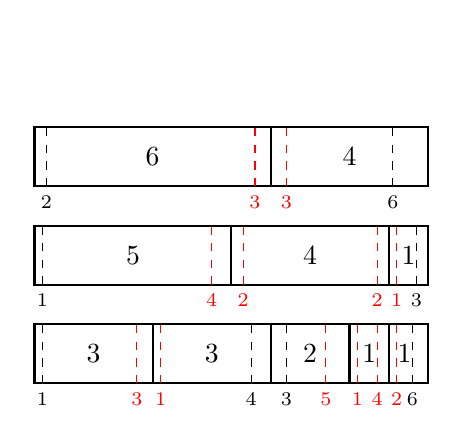
\begin{tikzpicture}
%\draw [help lines] (-1,-2) grid (13,5);
% 1=0.1, 2=0.15, 3=0.2, 4=0.25, 5=0.3
% 6, 5, 4, 4, 3, 3, 2, 1, 1, 1.

% BPP
\draw [thick] (0,0) rectangle (5,0.75);
\draw [thick] (0,1.25) rectangle (5,2);
\draw [thick] (0,2.5) rectangle (5,3.25);
\draw [thick, white] (0,3.75) rectangle (5,4.5);
 
% Bottom row, 3, 3, 2, 1 (1-3 X 1-4, 3-5 X 1-4 X 2-6)
\draw [thick] (1.5,0) -- (1.5,0.75);
\draw [thick] (3,0) -- (3,0.75);
\draw [thick] (4,0) -- (4,0.75);
\draw [thick] (4.5,0) -- (4.5,0.75);
\draw [dashed] (0.1,0) -- (0.1,0.75);
\draw [dashed, tRed] (1.3,0) -- (1.3,0.75);
\draw [dashed, tRed] (1.6,0) -- (1.6,0.75);
\draw [dashed] (2.75,0) -- (2.75,0.75);
\draw [dashed] (3.2,0) -- (3.2,0.75);
\draw [dashed, tRed] (3.7,0) -- (3.7,0.75);
\draw [dashed, tRed] (4.1,0) -- (4.1,0.75);
\draw [dashed, tRed] (4.35,0) -- (4.35,0.75);
\draw [dashed, tRed] (4.6,0) -- (4.6,0.75);
\draw [dashed] (4.8,0) -- (4.8,0.75);
\node [below] at (0.1,0) {\scriptsize{1}};
\node [below] at (1.3,0) {\textcolor{tRed}{\scriptsize{3}}};
\node [below] at (1.6,0) {\textcolor{tRed}{\scriptsize{1}}};
\node [below] at (2.75,0) {\scriptsize{4}};
\node [below] at (3.2,0) {\scriptsize{3}};
\node [below] at (3.7,0) {\textcolor{tRed}{\scriptsize{5}}};
\node [below] at (4.1,0) {\textcolor{tRed}{\scriptsize{1}}};
\node [below] at (4.35,0) {\textcolor{tRed}{\scriptsize{4}}};
\node [below] at (4.6,0) {\textcolor{tRed}{\scriptsize{2}}};
\node [below] at (4.8,0) {\scriptsize{6}};
\node at (0.75, 0.375) {3};
\node at (2.25, 0.375) {3};
\node at (3.5, 0.375) {2};
\node at (4.25, 0.375) {1};
\node at (4.7, 0.375) {1};

% Middle row, 5, 4, 1 (1-4 X 2-2 X 1-3)
\draw [thick] (2.5,1.25) -- (2.5,2);
\draw [thick] (4.5,1.25) -- (4.5,2);
\draw [dashed] (0.1,1.25) -- (0.1,2);
\draw [dashed, tRed] (2.25,1.25) -- (2.25,2);
\draw [dashed, tRed] (2.65,1.25) -- (2.65,2);
\draw [dashed, tRed] (4.35,1.25) -- (4.35,2);
\draw [dashed, tRed] (4.6,1.25) -- (4.6,2);
\draw [dashed] (4.85,1.25) -- (4.85,2);
\node [below] at (0.1,1.25) {\scriptsize{1}};
\node [below] at (2.25,1.25) {\textcolor{tRed}{\scriptsize{4}}};
\node [below] at (2.65,1.25) {\textcolor{tRed}{\scriptsize{2}}};
\node [below] at (4.35,1.25) {\textcolor{tRed}{\scriptsize{2}}};
\node [below] at (4.6,1.25) {\textcolor{tRed}{\scriptsize{1}}};
\node [below] at (4.85,1.25) {\scriptsize{3}};
\node at (1.25, 1.625) {5};
\node at (3.5, 1.625) {4};
\node at (4.75, 1.625) {1};

% Top row, 6, 4 (2-3 X 3-6)
\draw [thick] (3,2.5) -- (3,3.25);
\draw [dashed] (0.15,2.5) -- (0.15,3.25);
\draw [dashed, tRed] (2.8,2.5) -- (2.8,3.25);
\draw [dashed, tRed] (3.2,2.5) -- (3.2,3.25);
\draw [dashed] (4.55,2.5) -- (4.55,3.25);
\node [below] at (0.15,2.5) {\scriptsize{2}};
\node [below] at (2.8,2.5) {\textcolor{tRed}{\scriptsize{3}}};
\node [below] at (3.2,2.5) {\textcolor{tRed}{\scriptsize{3}}};
\node [below] at (4.55,2.5) {\scriptsize{6}};
\node at (1.5, 2.875) {6};
\node at (4, 2.875) {4};


\end{tikzpicture}

\end{document}